\chapter{Rnw example chapter}
\label{chap:rnw}





This document was generated on Wed Apr 13 18:01:10 2016.

As shown in Figure \ref{fig:some_fig} and in Table \ref{tab:rtab1} we can see that bla bla \citep{B}.


\begin{knitrout}
\definecolor{shadecolor}{rgb}{0.969, 0.969, 0.969}\color{fgcolor}\begin{figure}
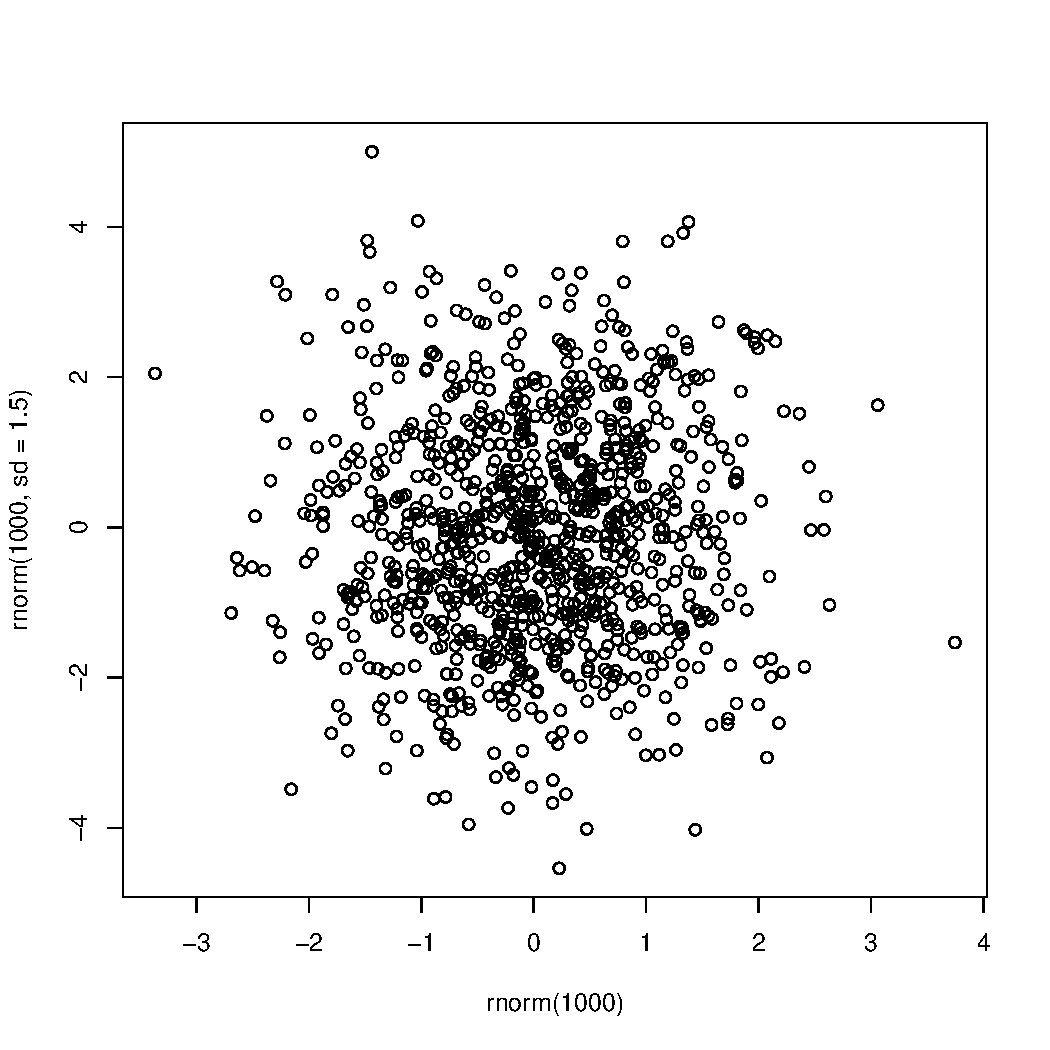
\includegraphics[width=\maxwidth]{figure/some_fig-1} \caption[{\bf Figure title } Rest of description]{{\bf Figure title } Rest of description}\label{fig:some_fig}
\end{figure}


\end{knitrout}






% latex table generated in R 3.3.0 by xtable 1.8-2 package
% Wed Apr 13 18:01:10 2016
\begin{table}[ht]
\centering
\begin{tabular}{rr}
  \hline
A & B \\ 
  \hline
  1 & -0.40 \\ 
    2 & -1.27 \\ 
    3 & -1.04 \\ 
    4 & 0.69 \\ 
    5 & 0.08 \\ 
    6 & 1.71 \\ 
    7 & 1.90 \\ 
    8 & 1.88 \\ 
    9 & 0.17 \\ 
   10 & -1.62 \\ 
   \hline
\end{tabular}
\caption{\bf{ Table title } Table description} 
\label{tab:rtab1}
\end{table}

